\chapter{Judges and Officials Rules}

\section{Hockey Director}

The Hockey Director is the head organizer and administrator of hockey events.
The Hockey Director is responsible for the logistics and equipment for the hockey competition.
The Hockey Director is in charge of keeping events running on schedule.

\section{Board of Referees}

\subsection{Members Of The Board Of Referees}
\begin{wrapfigure}{r}{0.5\textwidth}
\begin{center}
\includegraphics[scale=0.75]{referees}
\end{center}
\end{wrapfigure}
 The Board of Referees consists of:
\begin{itemize}
\item First Referee (1)
\item Second Referee (2)
\item Secretary (S)
\item Timer (T)
\end{itemize}

\subsection{The Referees}
The two Referees are positioned on opposite sides.
They try to stay close to the ball.
They should not ride a unicycle.
The clothes of the Referees must be of different color than those of the players.
Both Referees are responsible for checking all violations of the rules.
The first Referee has three additional tasks:
\begin{itemize}
\item The First Referee overrules the Second Referee, if they disagree.
\item The First Referee restarts the game after every interruption by a long blow of the whistle.
\item The First Referee drops the ball in for the face-off.
\end{itemize}

\subsection{The Secretary}
The Secretary sits at the desk and takes care that the scoreboard always shows the current score.
After a goal the Secretary seeks eye contact with the First Referee to check if the goal is declared valid or not.
After the end of the game the Secretary writes the final score into the report.

\subsection{The Timer}
The Timer checks the time of play with a stopwatch and/or with a score board.
The time is started whenever the Referee starts the game by blowing the whistle.
Each period is ended by the sound of the score board (e.g.\ horn, bell, gong) or the blowing of a whistle by the timer.
The Timer also stops the time whenever the Referee requests a time out.

\subsection{Before The Game}
Before the game, the Referees assemble all players on the field (including substitutes).
They check the following:
\begin{itemize}
\item Are the colors of the shirts of the players clearly different?
\item Do all players fulfill the safety rules for clothing (see section \ref{subsec:hockey_safety_clothing})?
\item Is the ball suitable?
\item Are the unicycles and sticks orderly, without sharp, pointed or protruding parts that might injure others?
\item They explain to the players how strictly they will interpret the rules.
\item If necessary, they tell the players how long the game will be and also if there is extended time in case of a draw.
\end{itemize}

\subsection{General}
The game is interrupted by a short and loud blow of the whistle.
If any players don't hear the whistle, it is necessary to blow the whistle again.
It is not possible to let the game continue after blowing the whistle.

The Referees should set the tone through their positive and calm appearance.
Decisions are explained upon request but they are not discussed with the players.
In an unclear situation, the Referees can ask the players before making a final decision.

Neither the Referees nor the Timer or Secretary may be distracted from the game.
Most of all, they must not talk with the spectators during the game.

If two violations of the rules occur back-to-back, only the first one is penalized.
Exception: Unsporting behavior should be penalized even after the game has been interrupted.

After a goal, the Referee waits until both teams are back in their own halves and ready to continue.
Only then, the first Referee starts the game by blowing the whistle.

To apply the advantage rule, the Referee makes the normal sign for a free shot with one arm pointing in the direction of play of the team who has the advantage.
In addition, the Referee may shout ``Advantage'' or ``Go ahead!'', but does not blow the whistle.
The end of advantage play should be signified, either by blowing the whistle to give a free shot for the original foul in the case where no advantage was gained, or by lowering the arm again and/or shouting ``Advantage over''.

After each interruption of the game the Referee briefly explains the decision.
In addition the corresponding hand sign is shown.

When two or more players fall and it is unclear whether a foul occurred, the Referees can interrupt the game and then continue it with a face-off.
This prevents more players being drawn into the situation.

The Referees suspend the game if an injury occurs.
Afterwards, a free shot is given to the team that was in possession of the ball at the time of the interruption.
If it is unclear who was in possession, the game is continued with a face-off.

If a referee is hit by the ball, the game is only interrupted if the contact has changed the course of play to benefit either team.
In this case, the game is resumed with a face-off.

\subsection{Referee Hand Signs}
\renewcommand{\arraystretch}{1.5}
\begin{longtable}{|c|p{10.8cm}|}

\hline %%%%%%%%%%%%%%%%%%%%%%%%%%%%%%%%%%%%%%%%%%%

\raisebox{-\height}[0mm][1.1\height]{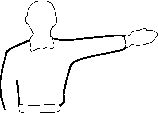
\includegraphics{hockey_foul}}
&
\textbf{``Free shot''}

Point with the extended arm in the direction of play.

This sign is also used to indicate the advantage rule.\\

\hline %%%%%%%%%%%%%%%%%%%%%%%%%%%%%%%%%%%%%%%%%%%

\raisebox{-\height}[0mm][1.1\height]{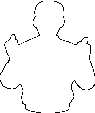
\includegraphics{hockey_washout}}
&
\textbf{``Face-off''}

Hold both thumbs up.\\

\hline %%%%%%%%%%%%%%%%%%%%%%%%%%%%%%%%%%%%%%%%%%%

\raisebox{-\height}[0mm][1.1\height]{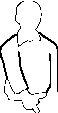
\includegraphics{hockey_6_50m}}
&
\textbf{``6.5\,m''}

Point with the index finger to the 6.5\,m point.\\

\hline %%%%%%%%%%%%%%%%%%%%%%%%%%%%%%%%%%%%%%%%%%%

\raisebox{-\height}[0mm][1.1\height]{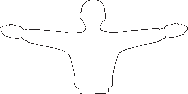
\includegraphics{hockey_nofoul}}
&
\textbf{``No Foul''}

Extend both arms horizontally.

This sign is used to indicate that there was no foul in a critical situation.
It is not used in conjunction with a blow of the whistle.\\

\hline %%%%%%%%%%%%%%%%%%%%%%%%%%%%%%%%%%%%%%%%%%%

\raisebox{-\height}[0mm][1.1\height]{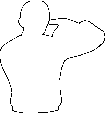
\includegraphics{hockey_timeout}}
&
\textbf{``Time out''}

Form the letter ``T'' with both hands.

The game is interrupted for example if a player is injured or if the spectators disturb the game.\\

\hline %%%%%%%%%%%%%%%%%%%%%%%%%%%%%%%%%%%%%%%%%%%

\raisebox{-\height}[0mm][1.1\height]{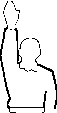
\includegraphics{hockey_goal}}
&
\textbf{``Goal''}

Point upwards vertically with one arm.

The Referees should check here that the secretary notes the goal.
To control this it may be useful for the Referees to write down the score themselves.\\

\hline %%%%%%%%%%%%%%%%%%%%%%%%%%%%%%%%%%%%%%%%%%%

\raisebox{-\height}[0mm][1.1\height]{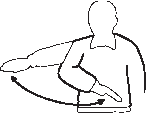
\includegraphics{hockey_nogoal}}
&
\textbf{``No goal''}

Move the flat hand horizontally (palm pointing down).

With this hand sign a goal shot is declared invalid.
This is for example the case if the ball was last touched by hand or arm, in case of a long shot, if the ball entered the goal through the net from the outside, or if the game had already been stopped before the ball entered the goal.
The Referees should check here that the Secretary does not inadvertently count the invalid goal.\\

\hline %%%%%%%%%%%%%%%%%%%%%%%%%%%%%%%%%%%%%%%%%%%

\raisebox{-\height}[0mm][1.1\height]{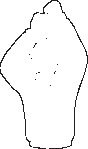
\includegraphics{hockey_highstick}}
&
\textbf{``High stick''}

Hold clenched fists next to each other above the head.\\

\hline %%%%%%%%%%%%%%%%%%%%%%%%%%%%%%%%%%%%%%%%%%%

\raisebox{-\height}[0mm][1.1\height]{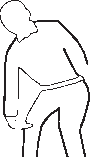
\includegraphics{hockey_sub}}
  &
\textbf{``SUB and SIB''}

Hit your shinbone with the edge of your hand.\\

\hline %%%%%%%%%%%%%%%%%%%%%%%%%%%%%%%%%%%%%%%%%%%

\raisebox{-\height}[0mm][1.1\height]{\includegraphics{hockey_obstacle}}
  &
\textbf{``Obstacle''}

Cross arms in front of the chest.\\

\hline %%%%%%%%%%%%%%%%%%%%%%%%%%%%%%%%%%%%%%%%%%%

\raisebox{-\height}[0mm][1.1\height]{\includegraphics{hockey_bodycontact}}
  &
\textbf{``Body contact''}

Strike the clenched fist of one hand into the open palm of the other hand directly in front of the chest.\\

\hline %%%%%%%%%%%%%%%%%%%%%%%%%%%%%%%%%%%%%%%%%%%

\raisebox{-\height}[0mm][1.1\height]{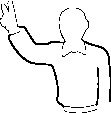
\includegraphics{hockey_2_min}}
&
\textbf{``Penalty box for 2 minutes''}

and also

\textbf{``Two consecutive plays with the hand''}

Spread and raise two fingers.\\

\hline %%%%%%%%%%%%%%%%%%%%%%%%%%%%%%%%%%%%%%%%%%%

\raisebox{-\height}[0mm][1.1\height]{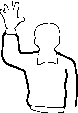
\includegraphics{hockey_5_min}}
  &
\textbf{``Penalty box for 5 minutes''}

Spread and raise five fingers.\\

\hline %%%%%%%%%%%%%%%%%%%%%%%%%%%%%%%%%%%%%%%%%%%


\end{longtable}
\renewcommand{\arraystretch}{1}
